\documentclass[10pt]{article}
\usepackage{fullpage,enumitem,amsmath,amssymb,graphicx,listings,tikz,bbm,xcolor}
\setlength{\parindent}{0pt}

\begin{document}

\begin{center}
{\Large \textbf{Homework 7: Car Tracking}}

\begin{tabular}{rl}
\\
Course: & CS 221 Spring 2019 \\
Name: & Bryan Yaggi
\end{tabular}
\end{center}

\section*{\normalsize Problem 1: Bayesian Network Basics}

First, let us look at a simplified version of the car tracking problem. For this problem only, let $C_t \in \{0,1\}$ be the actual location of the car we wish to observe at time step $t \in \{1,2,3\}$. Let $D_t \in \{0,1\}$ be a sensor reading for the location of that car measured at time $t$. Here's what the Bayesian network (it's an HMM, in fact) looks like:

\begin{center}
  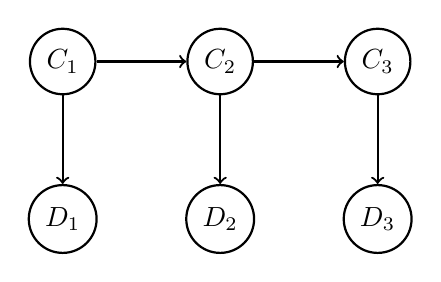
\begin{tikzpicture}
		\begin{scope}[every node/.style={circle,thick,draw}]
    		\node (C1) at (0,2) {$C_1$};
    		\node (C2) at (2,2) {$C_2$};
    		\node (C3) at (4,2) {$C_3$};
    		\node (D1) at (0,0) {$D_1$};
    		\node (D2) at (2,0) {$D_2$};
    		\node (D3) at (4,0) {$D_3$};
		\end{scope}
		\begin{scope}[every edge/.style={draw=black,thick}]
			\path [->] (C1) edge node {} (D1);	    		
    		\path [->] (C2) edge node {} (D2);
    		\path [->] (C3) edge node {} (D3);
    		\path [->] (C1) edge node {} (C2);
    		\path [->] (C2) edge node {} (C3);
		\end{scope}
	\end{tikzpicture}
\end{center}

The distribution over the initial car distribution is uniform; that is, for each value $c_1 \in \{0,1\}$:
$$p(c_1) = 0.5$$

The following local conditional distribution governs the movement of the car (with probability $\epsilon$, the car moves). For each $t \in \{2,3\}$:
$$p(c_t \mid c_{t-1}) = \begin{cases}
	\epsilon &\text{if} \ c_t \neq c_{t-1}\\
	1 - \epsilon &\text{if} \ c_t = c_{t-1}
\end{cases}$$

The following local conditional distribution governs the noise in the sensor reading (with probability $\eta$, the sensor reports the wrong position). For each $t \in \{1,2,3\}$:
$$p(d_t \mid c_t) = \begin{cases}
	\eta &\text{if} \ d_t \neq c_t\\
	1 - \eta &\text{if} \ d_t = c_t
\end{cases}$$

Below, you will be asked to find the posterior distribution for the car's position at the second time step ($C_2$) given different sensor readings.
\smallskip

Important: For the following computations, try to follow the general strategy described in lecture (marginalize non-ancestral variables, condition, and perform variable elimination). Try to delay normalization until the very end. You'll get more insight than trying to chug through lots of equations.

\begin{enumerate}[label=(\alph*)]

  \item Suppose we have a sensor reading for the second timestep, $D_2 = 0$. Compute the posterior distribution $\mathbb{P}(C_2 = 1 \mid D_2 = 0)$. We encourage you to draw out the (factor) graph.
  
  \begin{center}
	  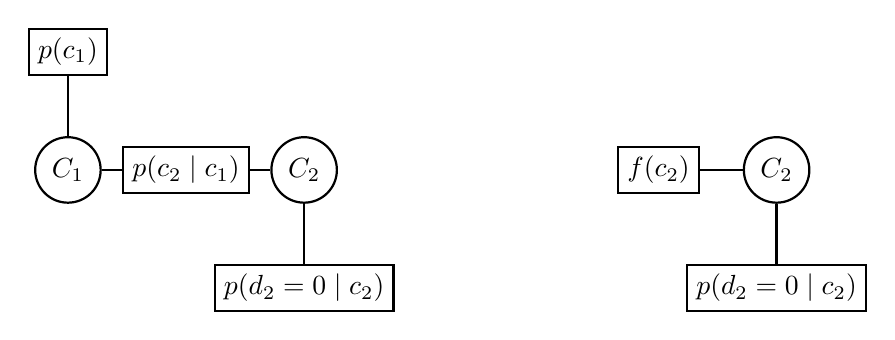
\begin{tikzpicture}
			\begin{scope}[every node/.style={circle,thick,draw}]
	    		\node (C11) at (0,3) {$C_1$};
	    		\node (C21) at (3,3) {$C_2$};
	    		\node (C22) at (9,3) {$C_2$};
			\end{scope}
			\begin{scope}[every node/.style={rectangle,thick,draw}]
	    		\node (f0) at (0,4.5) {$p(c_1)$};
	    		\node (f1) at (1.5,3) {$p(c_2 \mid c_1)$};
	    		\node (f21) at (3,1.5) {$p(d_2 = 0 \mid c_2)$};
	    		\node (f3) at (7.5,3) {$f(c_2)$};
	    		\node (f22) at (9,1.5) {$p(d_2 = 0 \mid c_2)$};
			\end{scope}
			\begin{scope}[every edge/.style={draw=black,thick}]
				\path [-] (f0) edge node {} (C11);	    		
	    		\path [-] (C11) edge node {} (f1);
	    		\path [-] (f1) edge node {} (C21);
	    		\path [-] (C21) edge node {} (f21);
	    		\path [-] (f3) edge node {} (C22);
	    		\path [-] (C22) edge node {} (f22);
			\end{scope}
		\end{tikzpicture}
	\end{center}

	\begin{align*}
	f(c_2) &= \sum_{c_1} p(c_1) p(c_2 \mid c_1) = \begin{cases}
	.5 (1 - \epsilon) + .5\epsilon = .5 &\text{if} \ c_2 = 0\\
	.5 \epsilon + .5 (1 - \epsilon) = .5 &\text{if} \ c_2 = 1
	\end{cases}\\
	\mathbb{P}(C_2 = c_2 \mid D_2 = 0) &\propto f(c_2) p(d_2 = 0 \mid c_2) = \begin{cases}
	.5(1 - \eta) &\text{if} \ c_2 = 0\\
	.5\eta &\text{if} \ c_2 = 1
	\end{cases}\\
	\mathbb{P}(C_2 = 1 \mid D_2 = 0) &= \eta
	\end{align*}
  
  \item Suppose a time step has elapsed and we got another sensor reading, $D_3 = 1$, but we are still interested in $C_2$. Compute the posterior distribution $\mathbb{P}(C_2 = 1 \mid D_2 = 0, D_3 = 1)$. The resulting expression might be moderately complex. We encourage you to draw out the (factor) graph.
  
  \begin{center}
	  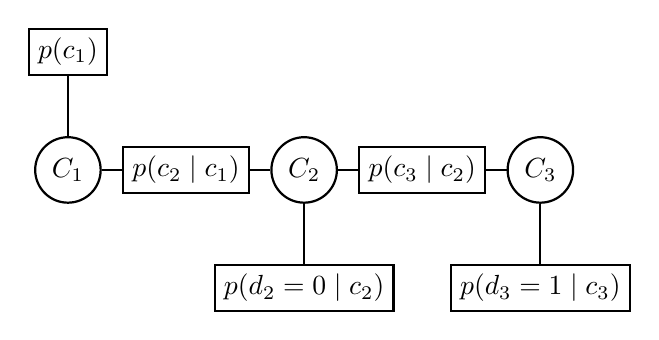
\begin{tikzpicture}
			\begin{scope}[every node/.style={circle,thick,draw}]
	    		\node (C1) at (0,3) {$C_1$};
	    		\node (C2) at (3,3) {$C_2$};
	    		\node (C3) at (6,3) {$C_3$};
			\end{scope}
			\begin{scope}[every node/.style={rectangle,thick,draw}]
	    		\node (f0) at (0,4.5) {$p(c_1)$};
	    		\node (f1) at (1.5,3) {$p(c_2 \mid c_1)$};
	    		\node (f2) at (3,1.5) {$p(d_2 = 0 \mid c_2)$};
	    		\node (f3) at (4.5,3) {$p(c_3 \mid c_2)$};
	    		\node (f4) at (6,1.5) {$p(d_3 = 1 \mid c_3)$};
			\end{scope}
			\begin{scope}[every edge/.style={draw=black,thick}]
				\path [-] (f0) edge node {} (C1);	    		
	    		\path [-] (C1) edge node {} (f1);
	    		\path [-] (f1) edge node {} (C2);
	    		\path [-] (C2) edge node {} (f2);
	    		\path [-] (C2) edge node {} (f3);
	    		\path [-] (f3) edge node {} (C3);
	    		\path [-] (C3) edge node {} (f4);
			\end{scope}
		\end{tikzpicture}
	\end{center}
	
	\begin{center}
	  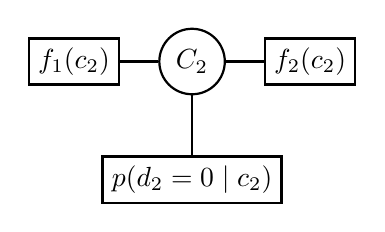
\begin{tikzpicture}
			\begin{scope}[every node/.style={circle,thick,draw}]
	    		\node (C2) at (3,3) {$C_2$};
			\end{scope}
			\begin{scope}[every node/.style={rectangle,thick,draw}]
	    		\node (f5) at (1.5,3) {$f_1(c_2)$};
	    		\node (f2) at (3,1.5) {$p(d_2 = 0 \mid c_2)$};
	    		\node (f6) at (4.5,3) {$f_2(c_2)$};
			\end{scope}
			\begin{scope}[every edge/.style={draw=black,thick}]
	    		\path [-] (f5) edge node {} (C2);
	    		\path [-] (C2) edge node {} (f2);
	    		\path [-] (C2) edge node {} (f6);
			\end{scope}
		\end{tikzpicture}
	\end{center}
	
	\begin{align*}
	f_1(c_2) &= \sum_{c_1} p(c_1) p(c_2 \mid c_1) = \begin{cases}
	.5 (1 - \epsilon) + .5\epsilon = .5 &\text{if} \ c_2 = 0\\
	.5 \epsilon + .5 (1 - \epsilon) = .5 &\text{if} \ c_2 = 1
	\end{cases}\\
	f_2(c_2) &= \sum_{c_3} p(c_3 \mid c_2) p(d_3 = 1 \mid c_3) = \begin{cases}
	(1 - \epsilon)\eta + \epsilon(1 - \eta) &\text{if} \ c_2 = 0\\
	\epsilon\eta + (1 - \epsilon)(1 - \eta) &\text{if} \ c_2 = 1
	\end{cases}\\
	\mathbb{P}(C_2 = c_2 \mid D_2 = 0, D_3 = 1) &\propto f_1(c_2) p(d_2 = 0 \mid c_2) f_2(c_2) = \begin{cases}
	.5(1 - \eta)((1 - \epsilon)\eta + \epsilon(1 - \eta)) &\text{if} \ c_2 = 0\\
	.5\eta(\epsilon\eta + (1 - \epsilon)(1 - \eta)) &\text{if} \ c_2 = 1
	\end{cases}\\
	\mathbb{P}(C_2 = 1 \mid D_2 = 0, D_3 = 1) &= \frac{\epsilon\eta^2 + (1 - \epsilon)(1 - \eta)\eta}{\epsilon\eta^2 + 2(1 - \epsilon)(1 - \eta)\eta + \epsilon(1 - \eta)^2}
	\end{align*}
		
	\item Suppose $\epsilon = 0.1$ and $\eta = 0.2$.
	\begin{enumerate}[label=(\roman*)]
		\item Compute and compare the probabilities $\mathbb{P}(C_2 = 1 \mid D_2 = 0)$ and $\mathbb{P}(C_2 = 1 \mid D_2 = 0, D_3 = 1)$. Give numbers, round your answer to 4 significant digits.
		
		\begin{align*}
		\mathbb{P}(C_2 = 1 \mid D_2 = 0) &= .2\\
		\mathbb{P}(C_2 = 1 \mid D_2 = 0, D_3 = 1) &= .4157
		\end{align*}
		
		\item How did adding the second sensor reading $D_3 = 1$ change the result? Explain your intuition for why this change makes sense in terms of the car positions and associated sensor observations.
		
		It increased the probability that $C_2 = 1$. Additional data is given that supports $C_2 = 1$. Since the probability that the position changes between timesteps is small, having the sensor reading $D_3 = 1$ makes it more likely that $C_2 = 1$. 
		
		\item What would you have to set $\epsilon$ while keeping $\eta = 0.2$ so that $\mathbb{P}(C_2 = 1 \mid D_2 = 0) = \mathbb{P}(C_2 = 1 \mid D_2 = 0, D_3 = 1)$? Explain your intuition in terms of the car positions with respect to the observations.
		
		$$\epsilon = .5$$
		
		This is effectively making it equally likely for $C_3$ to be 0 or 1 which makes knowing $D_3 = 1$ irrelevant.
		
	\end{enumerate}

\end{enumerate}

\section*{\normalsize Problem 2: Emission Probabilities}

\begin{enumerate}[label=(\alph*)]

  \item coding

\end{enumerate}

\section*{\normalsize Problem 3: Transition Probabilities}

\begin{enumerate}[label=(\alph*)]

  \item coding

\end{enumerate}

\section*{\normalsize Problem 4: Particle Filtering}

\begin{enumerate}[label=(\alph*)]

  \item coding
  
  \item coding  

\end{enumerate}

\section*{\normalsize Problem 5: Which Car is It?}

So far, we have assumed that we have a distinct noisy distance reading for each car, but in reality, our microphone would just pick up an undistinguished set of these signals, and we wouldn't know which distance reading corresponds to which car. First, let's extend the notation from before: let $C_{ti} \in \mathbb{R}^2$ be the location of the $i$-th car at the time step $t$, for $i = 1, \dots, K$ and $t = 1, \dots, T$. Recall that all the cars move independently according to the transition dynamics as before.
\smallskip 

Let $D_{ti} \in \mathbb{R}$ be the noisy distance measurement of the $i$-th car, which is now not observed. Instead, we observe the set of distances $D_t = \{D_{t1}, \dots, D_{tK}\}$ (assume that all distances are all distinct). Alternatively, you can think of $E_t = (E_{t1}, \dots, E_{tK})$ as a list which is a uniformly random permutation of the noisy distances $(D_{t1}, \dots, D_{tK})$. For example, suppose $K = 2$ and $T = 2$. Before, we might have gotten distance readings of 1 and 2 for the first car and 3 and 4 for the second car. Now, our sensor readings would be permutations of $\{1, 3\}$ and $\{2 ,4\}$. Thus, even if we knew the second car was distance 3 away at time $t = 1$, we wouldn't know if it moved farther (4 away) or closer (2 away) at time $t = 2$.

\begin{enumerate}[label=(\alph*)]

  \item Suppose we have $K = 2$ cars and one time step $T = 1$. Write an expression for the conditional distribution $\mathbb{P}(C_{11}, C_{12} \mid E_1 = e_1)$ as a function of the PDF of a Gaussian $p_{\mathcal{N}}(\nu; \mu, \sigma^2)$ and the prior probability $p(c_{11})$ and $p(c_{12})$ over car locations. Your final answer should not contain variables $d_{11}$, $d_{12}$.
  
  Remember that $p_{\mathcal{N}}(\nu; \mu, \sigma^2)$ is the probability of a random variable, $\nu$, in a Gaussian distribution with mean $\mu$ and standard deviation $\sigma^2$. 
  
  \begin{center}
	  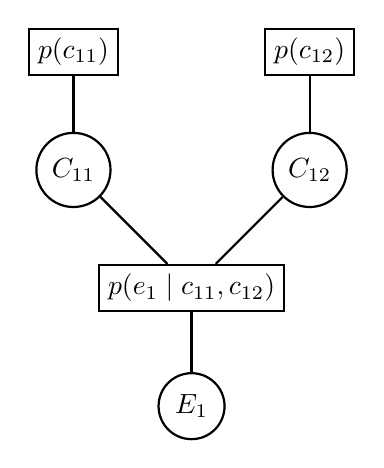
\begin{tikzpicture}
			\begin{scope}[every node/.style={circle,thick,draw}]
	    		\node (C11) at (0,0) {$C_{11}$};
	    		\node (C12) at (3,0) {$C_{12}$};
	    		\node (E1) at (1.5,-3) {$E_1$};
			\end{scope}
			\begin{scope}[every node/.style={rectangle,thick,draw}]
				\node (t0) at (0,1.5)	 {$p(c_{11})$};  		
	    		\node (t1) at (3,1.5) {$p(c_{12})$};
	    		\node (t2) at (1.5,-1.5) {$p(e_1 \mid c_{11}, c_{12})$};
			\end{scope}
			\begin{scope}[every edge/.style={draw=black,thick}]
				\path [-] (t0) edge node {} (C11);	    		
	    		\path [-] (t1) edge node {} (C12);
	    		\path [-] (C11) edge node {} (t2);
	    		\path [-] (C12) edge node {} (t2);
	    		\path [-] (t2) edge node {} (E1);
			\end{scope}
		\end{tikzpicture}
	\end{center}
	
	\begin{align*}
	\mathbb{P}(C_{11}, C_{12} \mid E_1 = e_1) &\propto p(c_{11}) p(c_{12}) (p(e_1 = \{ e_{11}, e_{12} \} \mid c_{11}, c_{12}) + p(e_1 = \{ e_{12}, e_{11} \} \mid c_{11}, c_{12}))\\
	p(e_1 = \{ e_{11}, e_{12} \} \mid c_{11}, c_{12}) &\propto p_{\mathcal{N}}(e_{11}; \lVert a_1 - c_{11} \rVert, \sigma^2) p_{\mathcal{N}}(e_{12}; \lVert a_1 - c_{12} \rVert, \sigma^2)\\
	p(e_1 = \{ e_{12}, e_{11} \} \mid c_{11}, c_{12}) &\propto p_{\mathcal{N}}(e_{12}; \lVert a_1 - c_{11} \rVert, \sigma^2) p_{\mathcal{N}}(e_{11}; \lVert a_1 - c_{12} \rVert, \sigma^2)\\
	\mathbb{P}(C_{11}, C_{12} \mid E_1 = e_1) &\propto p(c_{11}) p(c_{12}) (p_{\mathcal{N}}(e_{11}; \lVert a_1 - c_{11} \rVert, \sigma^2) p_{\mathcal{N}}(e_{12}; \lVert a_1 - c_{12} \rVert, \sigma^2)\\
	&+ p_{\mathcal{N}}(e_{12}; \lVert a_1 - c_{11} \rVert, \sigma^2) p_{\mathcal{N}}(e_{11}; \lVert a_1 - c_{12} \rVert, \sigma^2))
	\end{align*}
  
  \item Assuming the prior $p(c_{1i})$ is the same for all $i$, show that the number of assignments for all $K$ cars $(c_{11}, \dots, c_{1K})$ that obtain the maximum value of $\mathbb{P}(C_{11} = c_{11}, \dots, C_{1K} = c_{1K} \mid E_1 = e_1)$ is at least $K!$.
  
	Since the prior is the same for each car, each permutation of the initial assignment of observations to cars is also a solution. The total number of valid assignments is therefore $K!$.  
  
  \item For general $K$, what is the treewidth corresponding to the posterior distribution over all $K$ car locations at all $T$ time steps conditioned on all the sensor readings:
  $$\mathbb{P}(C_{11} = c_{11}, \dots, C_{1K} = c_{1K} , \dots, C_{T1} = c_{T1}, \dots, C_{TK} = c_{TK} \mid E_1 = e_1, \dots, E_T = e_T)$$

	The following factor graph shows 2 timesteps:
	
	\begin{center}
	  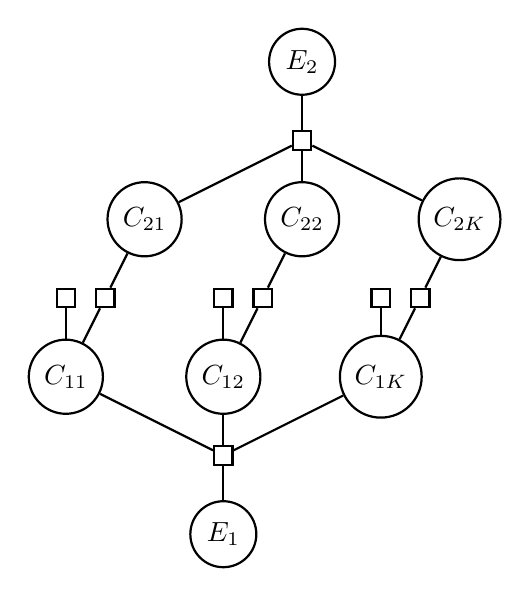
\begin{tikzpicture}
			\begin{scope}[every node/.style={circle,thick,draw}]
	    		\node (C11) at (0,0) {$C_{11}$};
	    		\node (C12) at (2,0) {$C_{12}$};
	    		\node (C1K) at (4,0) {$C_{1K}$};
	    		\node (E1) at (2,-2) {$E_1$};
	    		\node (C21) at (1,2) {$C_{21}$};
	    		\node (C22) at (3,2) {$C_{22}$};
	    		\node (C2K) at (5,2) {$C_{2K}$};
	    		\node (E2) at (3,4) {$E_2$};
			\end{scope}
			\begin{scope}[every node/.style={rectangle,thick,draw}]
				\node (t0) at (0,1)	 {};  		
	    		\node (t1) at (2,1) {};
	    		\node (t2) at (4,1) {};
	    		\node (t3) at (2,-1) {};
	    		\node (t7) at (3,3) {};
	    		\node (t8) at (.5,1) {};
	    		\node (t9) at (2.5,1) {};
	    		\node (t10) at (4.5,1) {};
			\end{scope}
			\begin{scope}[every edge/.style={draw=black,thick}]
				\path [-] (t0) edge node {} (C11);	    		
	    		\path [-] (t1) edge node {} (C12);
	    		\path [-] (t2) edge node {} (C1K);
	    		\path [-] (C11) edge node {} (t3);
	    		\path [-] (C12) edge node {} (t3);
	    		\path [-] (C1K) edge node {} (t3);
	    		\path [-] (t3) edge node {} (E1);
	    		\path [-] (C21) edge node {} (t7);
	    		\path [-] (C22) edge node {} (t7);
	    		\path [-] (C2K) edge node {} (t7);
	    		\path [-] (t7) edge node {} (E2);
	    		\path [-] (C11) edge node {} (t8);
	    		\path [-] (t8) edge node {} (C21);
	    		\path [-] (C12) edge node {} (t9);
	    		\path [-] (t9) edge node {} (C22);
	    		\path [-] (C1K) edge node {} (t10);
	    		\path [-] (t10) edge node {} (C2K);
			\end{scope}
		\end{tikzpicture}
	\end{center}
	
	The treewidth is $K$ as seen in the graph.
  \iffalse
  \item \textbf{[Extra Credit]} Now suppose you change your sensors so that at each time step $t$, they return the list of exact positions of the $K$ cars, but shifted (with wrap around) by a random amount. For example, if the true car positions at time step 1 are $c_{11}=1$, $c_{12}=3$, $c_{13}=8$, $c_{14}=5$, then $e_1$ would be $[1,3,8,5]$, $[3,8,5,1]$, $[8,5,1,3]$, or $[5,1,3,8]$, each with probability $\frac{1}{4}$. Describe an efficient algorithm for computing $p(c_{ti} \mid e_1, \dots, e_T)$ for any time step $t$ and car $i$. Your algorithm should not be exponential in $K$ or $T$.
	\fi
\end{enumerate}

\end{document}
